\documentclass[../main.tex]{subfiles}
\graphicspath{{figures/}{../figures/}}

\begin{document}
% \todo[color=green!30]{完成问题二模型的求解(sections/q2\_solution)}

利用模拟退火算法进行求解,最终筛选最优解,具体步骤如下:

\textbf{步骤1$\,\,$设定初始参数}

根据题目要求和经验,设定干扰弹发射角度、速度及投放时间等初始参数。

按照上述算法思路,利用Python求解得当$FY1$的飞行方向与$x$轴正方向的夹角$\alpha$为3.13$rad$(逆时针为真),飞行速度为109.78$m/s$,烟雾弹投放位置为(17722.061437,0.903555,1800.000000),烟雾弹起爆位置为(17335.661803,5.383153,1739.287040)时,遮蔽时间最长为4.602140$s$。

\textbf{步骤3 $\,\,$离散化时间轴}

将导弹飞行时间段划分为细小的时间步长,便于逐点判断遮蔽状态。

\textbf{步骤4 $\,\,$遍历时间点并判断遮蔽}

对每个时间点,计算干扰弹位置,结合导弹与目标几何关系,判断是否满足有效遮蔽条件。

\textbf{步骤5 $\,\,$统计总遮蔽时间}

收集所有满足遮蔽条件的时间点,累加得到总有效遮蔽时间。

\textbf{步骤6 $\,\,$构建优化目标函数}

以总遮蔽时间作为目标函数值,供优化算法调用。

 \textbf{步骤7 $\,\,$应用模拟退火算法}
 
 通过迭代生成新参数解,依据目标函数值变化和Metropolis准则接受或拒绝新解。\\
    Metropolis准则:以一定的概率接受一个新状态,即使这个新状态的能量(或目标函数值)比当前状态更低。这有助于算法跳出局部最优解,探索更广阔的状态空间。本代码中选择的比较值是\(\exp(\text{score\_diff} / \text{temp})\)。当新解更大时,选用新解;新解更小时,以\(\exp(\text{score\_diff} / \text{temp})\)的概率选用新解。

\textbf{步骤8 $\,\,$逐步优化并收敛}

随着迭代进行,不断更新最优参数组合,使有效遮蔽时间逐渐增加,最终趋于稳定最优值。
\begin{figure}[H]
\centering
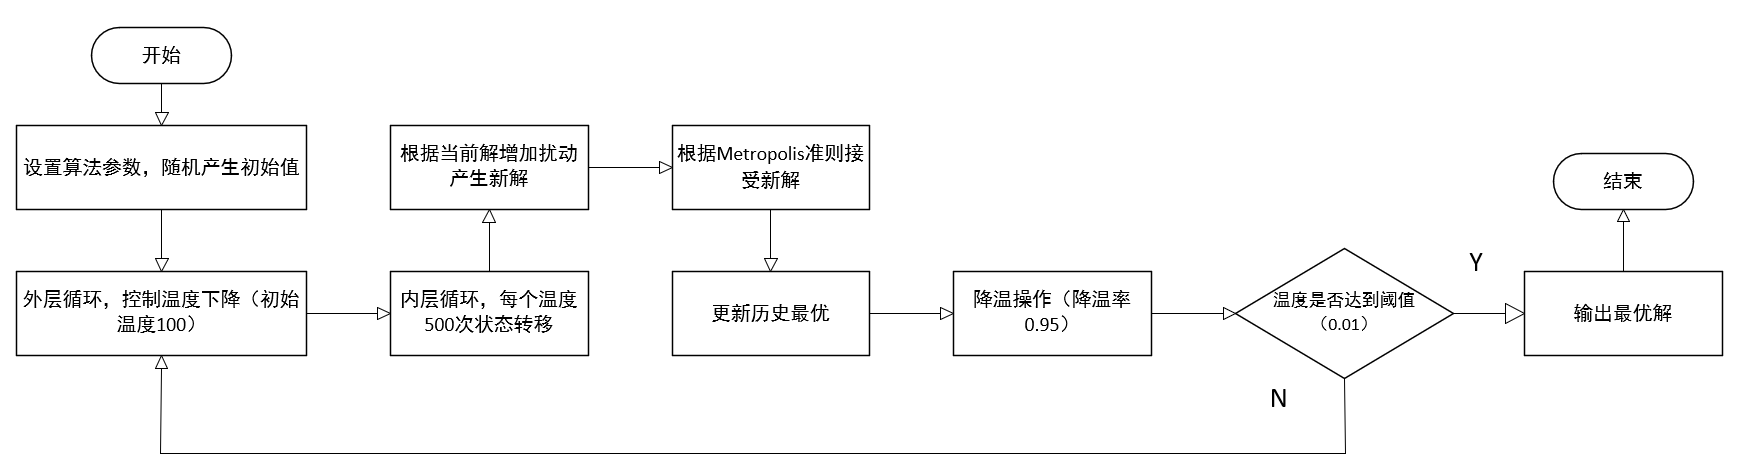
\includegraphics[scale=0.35]{问题二模型求解流程图.png}
\caption{问题二模型求解流程图}
\label{图2}
\end{figure}

按照上述算法思路,利用Python求解得







\end{document}